\chapter{Introduction}

The current document defines the package \multiVone of \sbmlLthreeVone. 

\section{Graphical and typographical conventions}

We use the following typographical conventions to distinguish objects and data types from other entities:

\begin{itemize}
 \item[\class{Class}:] Names of classes begin with a capital letter and are printed in a bold, sans-serif typeface. 
 \item[\attribute{attribute}:] Names of attributes begin with a lowercase letter and are printed in a bold, italic, sans-serif typeface. 
 \item[\cdata{value}:] CDATA (character data (see \url{http://en.wikipedia.org/wiki/CDATA})), that is the textual content of an element or the value of an attribute, is printed in a italic, sans-serif typeface.
 \item[\xmlcode{code}:] Examples of XML code are printed in monotype typeface. 
\end{itemize}

Some \class{SpeciesTypes} can represent binding sites. Those binding sites can be linked to other binding sites. In this document, a binding site can be represented in four different contexts:\\[\baselineskip]

\begin{tabular}{m{0.7\textwidth} m{0.3\textwidth}}
 A binding site declared as explicitly unbound is represented with a white background.& 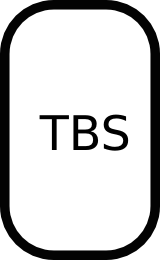
\includegraphics{figs/pngs/unbound.png} \\
 A binding site declared as either bound or unbound is represented with a grey background.& 
\includegraphics{figs/pngs/dunno.png} \\
 A binding site declared as bound to another undefined binding site is represented with a black background. & 
\includegraphics{figs/pngs/generic.png} \\
 A binding site bound declared as bound to a defined binding site is represented with a black background and a black edge linking it to the other binding site. &  
\includegraphics{figs/pngs/specific.png} \\
\end{tabular}

Throughout the text, the American spelling is used rather than the British one.

\section{Motivation}

This package \emph{multi} addresses two different --- though related --- problems, commonly encountered when trying to model biological processes:

\begin{itemize}
 \item The representation of entities that can exist under different states affecting their behaviours (multi-state entities). Those entities carry state features, sometimes many of them, each able to take different values. This  may result in a combinatorial explosion of alternative states taken by the entities.
\item The creation and behaviour of complexes made up of different components (multi-component entities). The rules of assembly may lead to an unbounded list of species, with the number of components and their topology impossible to precise before the simulation. 
\end{itemize}

As a simple example of multi-state multi-component entity, let's consider a ligand-gated ion channel with only one feature, the \cdata{pore}, that can adopt three different values, \cdata{closed}, \cdata{opened} and \cdata{desensitized}. In addition to this state feature, the channel can be bound to a scaffold through an \cdata{anchor}. 

%\begin{wrapfigure}{l}{60mm}
%  \includegraphics[width=58mm]{figs/pngs/IMG_2016.JPG}
%  \caption{How to bite}
%  \label{bite1}
%\end{wrapfigure}

%\begin{wrapfigure}{r}{5cm}
%  \begin{center}
%    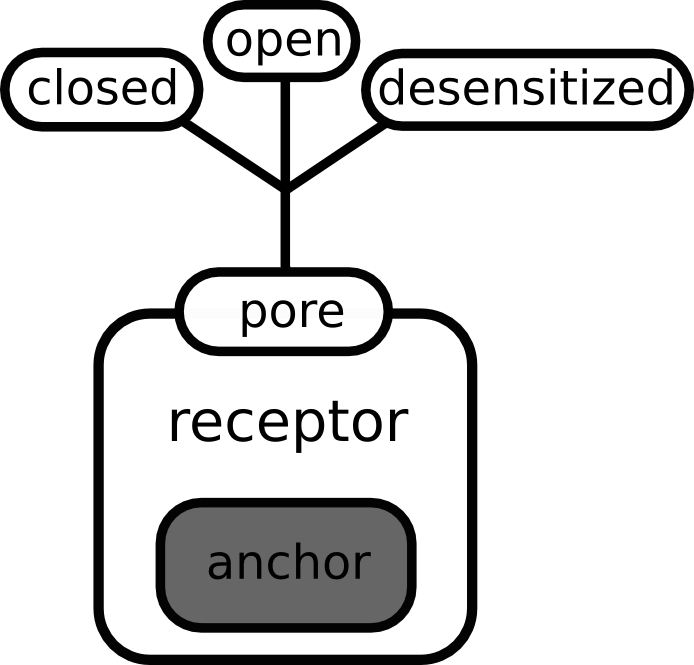
\includegraphics[width=4.8cm]{figs/pngs/st_receptor.png}
%  \end{center}
%  \caption{A gull}
%\end{wrapfigure}


%\begin{wrapfigure}{r}{0.5\textwidth}
% \begin{center}
%  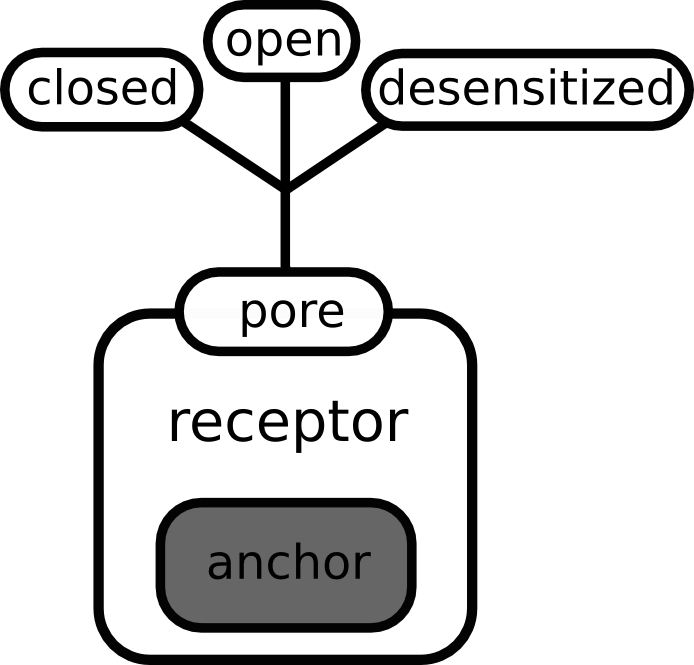
\includegraphics[width=0.48\textwidth]{figs/pngs/st_receptor.png}
%  \end{center}
%\caption{Example of a molecular entity carrying a multi-valued variable and containing another entity.}
%\end{wrapfigure}

\begin{figure}[H]
 \begin{center}
  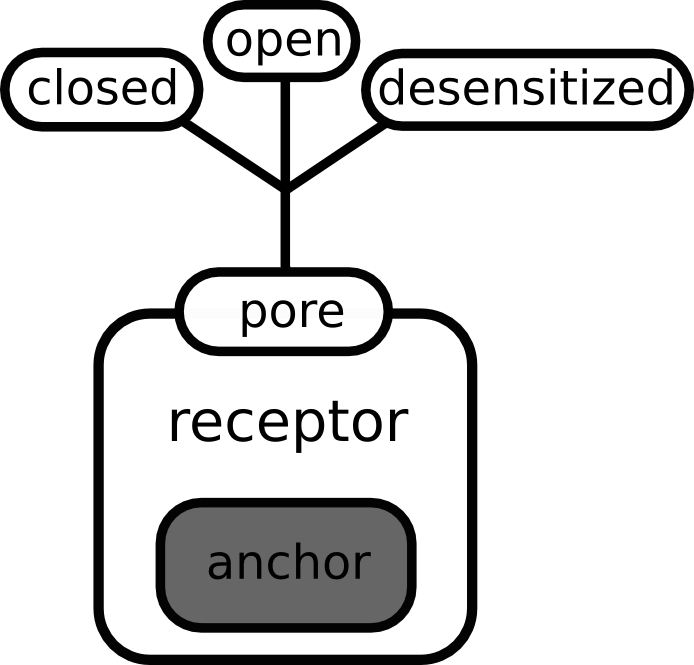
\includegraphics[scale=1]{figs/pngs/st_receptor.png}
\caption{Example of a molecular entity carrying a multi-valued variable and containing another entity.}
\label{fig:st_receptor}
  \end{center}
\end{figure}

Taking into account the different values for the state feature, plus the status of the anchoring site (bound or not), this receptor can exist under six different states:\\[\baselineskip] 

\begin{minipage}[c]{2in}
\noindent 
{free, closed}\\
{free, open}\\
{free, desensitized}\\
{anchored, closed}\\
{anchored, open}\\
{anchored, desensitized}\\
\end{minipage}

With the SBML core, any reaction involving the receptor, such as binding to a ligand, will have to be written six times. However, some of the state features and/or bonds may not affect the binding of the ligand, but the reactions have to be enumerated nevertheless, if we want to keep track of all the populations. Writing all the possibilities can be in the best case just exhausting, and in the worst case plainly impossible due to the combinatorial explosion. If an entity possesses 4 bivalued features and 2 trivalued features, the number of possible state is 24x32. A dodecamer of CaMKII with 5 different characteristics taking two values (e.g. activity, binding to calmodulin and to ATP, phosphorylations on threonin 286 and 306) exhibits 60 state features, and consequently a billion of billion possible states. Writing such a model by enumerating all possible states and reactions is plainly impossible, and one needs a way to describe only the relevant states of this species rather than all the possible ones.

Another problem addressed by the package \emph{multi} is the unbounded list of multi-component entities. Let's imagine a situation where we would like to model the growth of microtubules from dimers of tubulin. We cannot possibly enumerate all the possible microtubules of different lengths. Furthermore, the length of a microtubule does not affect the rate with which a new dimer of tubulin is incorporated. The only thing we need to encode is the binding between a tubulin dimer incorporated in a microtubule and a free tubulin dimer. 

\begin{figure}[H]
\begin{center}
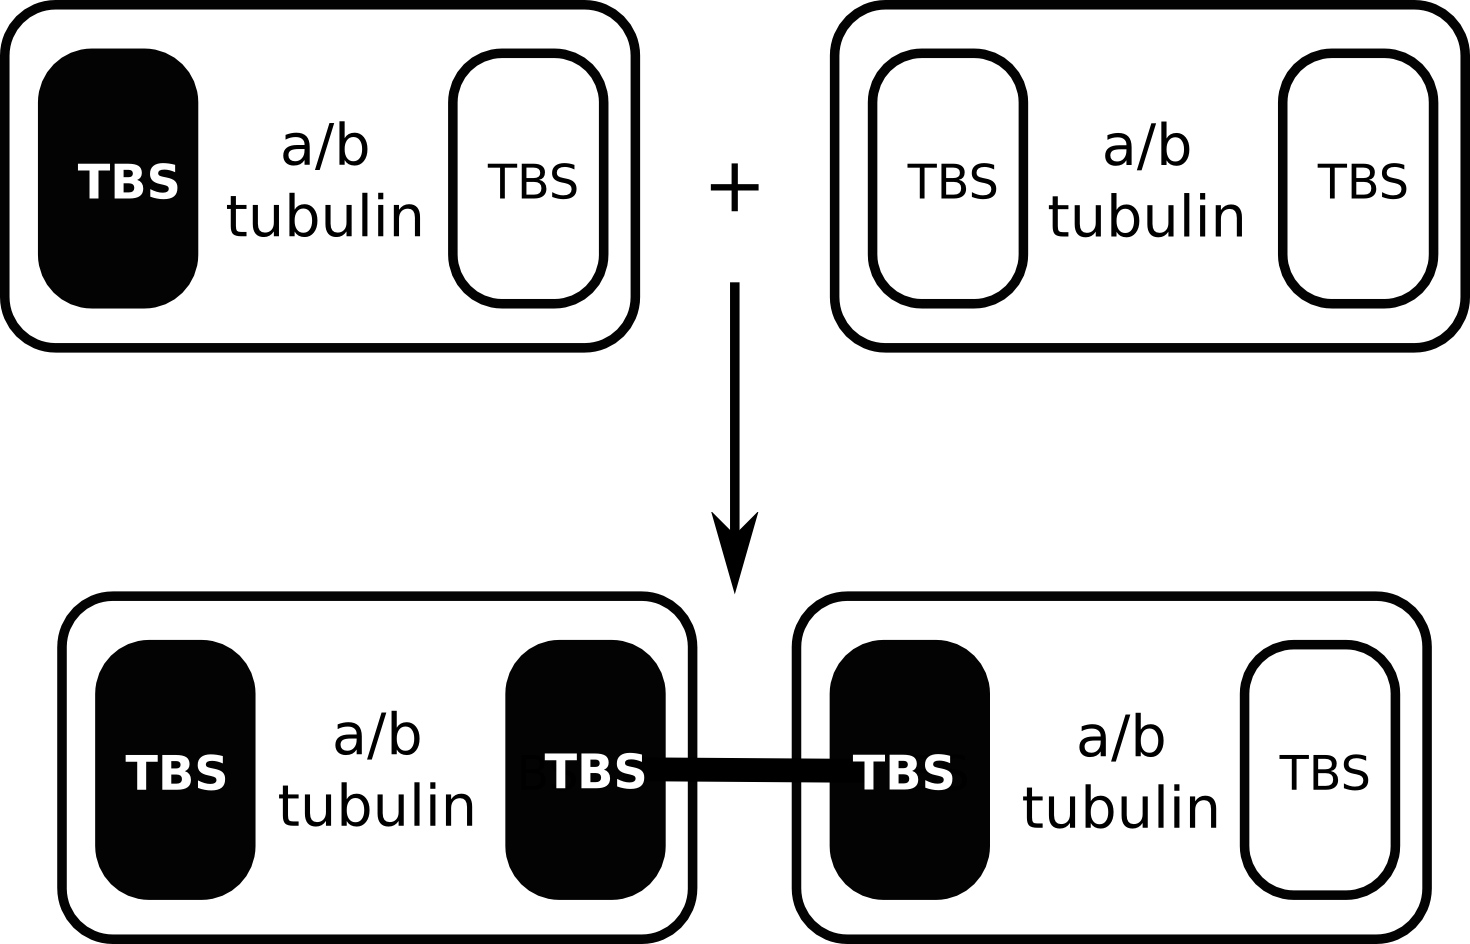
\includegraphics{figs/pngs/microtubule.png}
\caption{Example of a reaction involving entities with undefined binding status.}
\label{fig:microtubule}
\end{center}
\end{figure}

In the schema above, the grey binding site is either bound or unbound, and it can be bound to another tubulin dimer or a microtubule containing 100 tubulin dimers.

To handle the problems described above a field of modeling was developed, called rule-based modeling \citep{Hlavacek:2006}. The main idea of rule-based modeling is to write down the rules that reactions must obey rather than the reactions themselves. And example of language used to describe rule-based models in biology is BioNetGen \citep{Blinov:2004}. Another approach to avoid the combinatorial explosion of possible cases, is to use multi-agent modeling, where one represent all the interacting entities individually rather than pools. It the number of possible cases exceeds the number of entities, this method, otherwise verbose, become parsimonious. Example of multi-agent software used in biology are StochSim \citep{MortonFirth:1998,Lenov:2001} and Simmune \citep{MeierSchellersheim:2001,MeierSchellersheim:2006}. 

The graphical equivalent of the package \multiVone of \sbmlLthreeVone is the SBGN Entity Relationship language.

Finally, the package \emph{multi} permit to encode entities that are made of components belonging to different compartments. Those entities cannot be species, since a species is attached to a single compartment, and the compartments in \sbmlLthreeVone are not overlapping. In \emph{multi}, species types, representing species attached to different compartments, can be linked.  

\section{Past work on this problem or similar topics}

Proposals for supporting multistates and multicomponent species have a long history in SBML. Here is a reconstruction in chronological order:

\begin{itemize}
 \item Andrew Finney was probably the first to formulate, in March 2001, proposed SBML extensions to support complex species, to be able to cover \link{http://sbml.org/images/5/5a/Multistates_Finney-16Mar2001.pdf}{multistates species} and \link{http://sbml.org/images/b/ba/Multicomponents_Finney_14March2001.pdf}{species made up of graphs of components}, as part of a collection of proposals for new SBML development. At the \link{http://sbml.org/Events/Workshops/The_3rd_Workshop_on_Software_Platforms_for_Systems_Biology}{3\textsuperscript{rd} Workshop on Software Platforms for Systems Biology} in June 2001, Nicolas Le Nov\`ere gave a presentation entitled \link{http://sbml.org/images/1/1b/Lenovere.pdf}{Multistate molecules and complex objects} proposing to extend Andrew's multistate proposal. 

\item Nicolas Le Novère and Tom Shimizu came up in July 2001 with an \link{http://sbml.org/images/4/4b/Multistates_LeNovere_06July2001.txt.zip}{alternative proposal} for encoding and using states in SBML. A sligthly extended and corrected version of this proposal presented by Nicolas at the \link{http://sbml.org/Events/Workshops/The_5th_Workshop_on_Software_Platforms_for_Systems_Biology}{5\textsuperscript{th} Workshop on Software Platforms for Systems Biology} in July 2002. Nicolas Le Novère, Tom Shimizu and Andrew Finney published a \link{http://sbml.org/images/3/3c/Multistates_LeNovere_11December2002.pdf}{complete description of this extension} in December 2002. 

 \item In March 2004, before the \link{http://sbml.org/Events/Hackathons/The_2nd_SBML_Hackathon}{2\textsuperscript{nd} SBML hackathon}, Andrew Finney published an \link{http://sbml.org/images/6/67/CplxSpecies_Finney-31Mar2004.pdf}{updated proposal} to encode complex species made up of several components. Planed as an extension for SBML Level 3, the document also described SpeciesTypes that would later be incorporated to SBML Level 2, from version 2 onward. 

 \item In October 2004, Michael Blinov published, together with Jim Fader, Byron Goldstein, Andrew Finney and Bill Hlavacek, \link{http://sbml.org/images/1/17/CplxSpecies_Blinov-06Oct2004.pdf}{an alternative proposal} for encoding multi-component species, that also contained some possibilities of encoding multistate features. 

 \item Anika Oellrich started to implement a new SBML L2 support for StochSim in spring 2007, storing multistate information in proprietary annotations. This led in June 2007 to a \link{http://sbml.org/images/5/54/Multistates_LeNovere_23June2007.pdf}{proposal for Level 3} by Le Nov\`ere and Oellrich, meant to work in conjunction with 2004 Finney's multicomponents proposal. The proposal was presented at the \link{http://sbml.org/images/a/a4/20071005-lenovere-statevariables.pdf}{12\textsuperscript{th} SBML forum meeting}. A \link{http://sbml.org/images/4/4b/Multistates_LeNovere_06December2007.pdf}{light correction} was published in December 2007. 

 \item Also at the 12\textsuperscript{th} SBML forum meeting, Michael Blinov presented an \link{http://sbml.org/images/2/2a/20071005-blinov-sbml3rbm.pdf}{updated version of his proposal}. He later published two proposals for SBML L3, one with a \link{http://sbml.org/images/9/96/Blinov-sbml3-2007-06-12.pdf}{hierarchical speciesTypes} structure and one with a \link{http://sbml.org/images/0/0f/Blinov-sbml3-2007-06-08.pdf}{non-hierarchical speciesTypes} structure. 

 \item On December 6 and 7 2007, an \link{http://sbml.org/Events/Other_Events/SBML_Multicomponent_\%26_Multistate_Workshop_2007}{SBML Focused Videoconference} was held, which launched the effort to develope the Level 3 package multi. 
\end{itemize}



